 
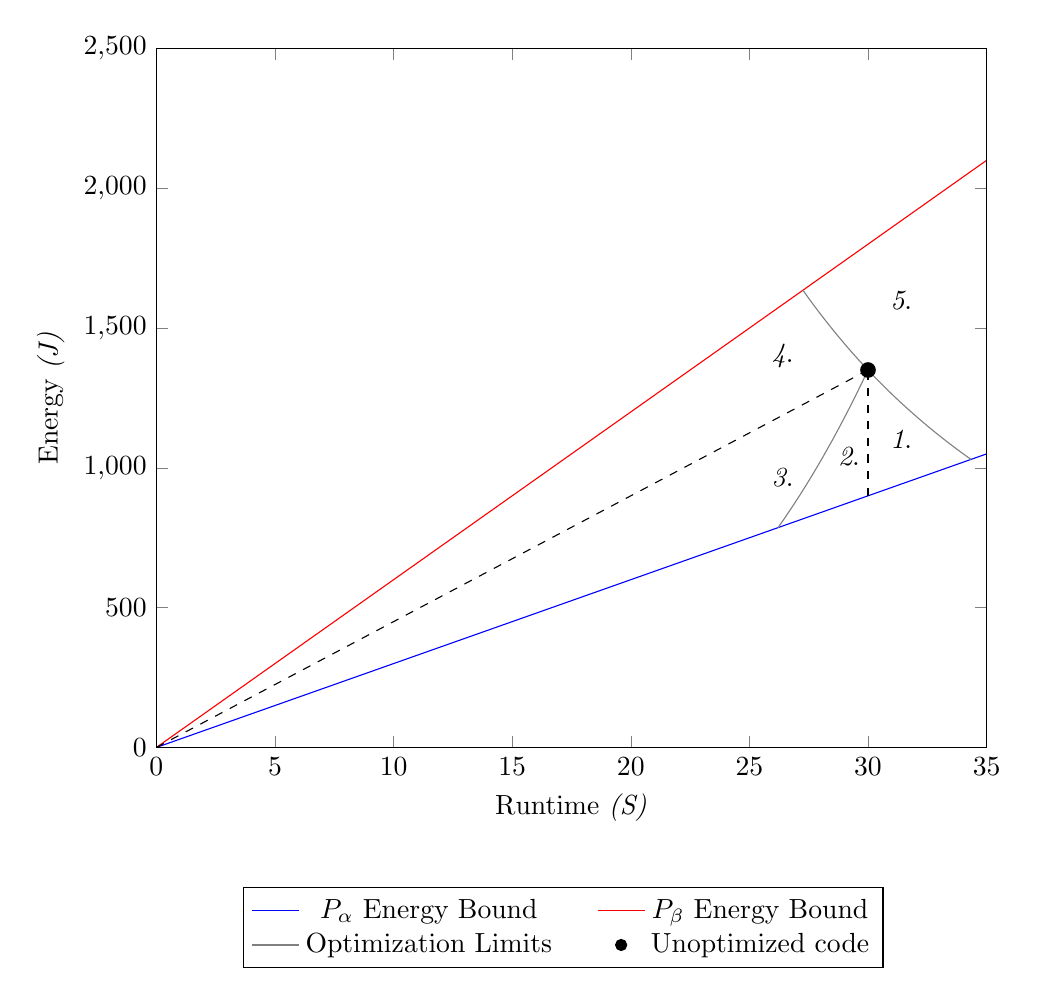
\begin{tikzpicture}
  \begin{axis}[no markers, ylabel={Energy \emph{(J)}}, xlabel={Runtime \emph{(S)}}, axis on top,
    ymin=0, ymax=2500,
    xmin=0, xmax=35,
    width=\linewidth,
    legend style={at={(0.49,-0.2)}, anchor=north,legend columns=2, /tikz/every even column/.append style={column sep=0.5cm}}
    ]

    \pgfmathsetmacro{\baseline}{30}
    \pgfmathsetmacro{\roofline}{60}
    \pgfmathsetmacro{\power}{(\baseline + \roofline) / 2}
    \pgfmathsetmacro{\seconds}{30}
    \pgfmathsetmacro{\energy}{\power * \seconds}
    \pgfmathsetmacro{\baseenergy}{\baseline * \seconds}


    \addplot[domain=\pgfkeysvalueof{/pgfplots/xmin}:\pgfkeysvalueof{/pgfplots/xmax}, blue] {\baseline * x};
    \addlegendentry{$P_{\alpha}$ Energy Bound} 


    \addplot[domain=\pgfkeysvalueof{/pgfplots/xmin}:\pgfkeysvalueof{/pgfplots/xmax}, red] {\roofline * x};
    \addlegendentry{$P_{\beta}$ Energy Bound}

    %ED2P boundaries
    \addlegendentry{Optimization Limits} 

    \addplot[domain=27.25680:34.34143, gray, forget plot] { (\power * \seconds^3) / ((x)^2)};
    \addplot[domain=26.2074:\seconds, gray] { (\power / \seconds^3) * x^4}; % Power time same ratio

    \addlegendimage{only marks, mark=o}
    \addlegendentry{Unoptimized code}


    \addplot[domain=\pgfkeysvalueof{/pgfplots/xmin}:\seconds, dashed] {\power * x};
    \draw[dashed] ({axis cs:\seconds,0}|-{axis cs:0,\baseenergy}) -- ({axis cs:\seconds,0}|-{axis cs:0,\energy});

    \node[circle,fill,inner sep=2pt] at (axis cs:\seconds,\energy) {};
    \node at (axis cs:31.4,1100) {\textit1.};
    \node at (axis cs:29.2,1040) {\textit2.};
    \node at (axis cs:26.4,965) {\textit3.};
    \node at (axis cs:26.4,1400) {\textit4.};
    \node at (axis cs:31.4,1600) {\textit5.};
      
 \end{axis}
\end{tikzpicture}
